\chapter{Умножение и деление}

\section{Умножение двух двухбитных чисел}

В этой главе мы попробуем с помощью сумматора
выполнять операцию умножения.
Схемы для умножения чисел нужной разрядности получаются намного сложнее схем для сложения,
поэтому такого модуля в конструкторе нет.

Для простоты уменьшим разрядность входных данных до двух бит и
посмотрим, что получится, когда мы умножаем два двухбитных числа
$a_1a_0$ и $b_1b_0$:

$$
\begin{array}{cccc}
     &  & a_1 & a_0 \\
& \times  & b_1 & b_0 \\ \hline
  & & a_1 \cdot b_0 & a_0 \cdot b_0 \\
+ & a_1 \cdot b_1 & a_0 \cdot b_1 & \\ \hline
& a_1 \cdot b_1 & a_0 \cdot b_1 + a_1 \cdot b_0 & a_0 \cdot b_0 \\
\end{array}
$$

Например, для чисел $10$ и $11$ получится так:

$$
\begin{array}{cccc}
     &  & 1 & 0 \\
& \times  & 1 & 1 \\ \hline
  & & 1 & 0 \\
+ & 1 & 0 & \\ \hline
& 1 & 1 & 0 \\
\end{array}
$$

Очень удобно, что мы работаем с битовыми представлениями чисел.
Ведь тогда арифметическое умножение на однобитное число совпадает
с логическим умножением каждого бита на это однобитное число:

$$a_1a_0 \cdot b_0 = (a_1\cdot b_0)0 + (a_0 \cdot b_0) = (a_1\ \mbox{\&}\ b_0)0 + (a_0\ \mbox{\&}\ b_0) = a_1a_0\ \mbox{\&}\ b_0b_0$$.

В отличие от сложения,
никакого переноса здесь не возникает, что несколько упрощает схему.
Поэтому вычислить эти частичные произведения можно с помощью одного модуля
логических операций, так как он работает с четырьмя битами за раз.

Только сначала нужно <<размножить>> биты операнда $b$ с помощью коммутационной матрицы.

Выходы с модуля <<И>> нужно подать на сумматор. Только два бита
умноженные на $b_0$ остаются на месте и подаются на первый вход сумматора, а
умноженные на $b_1$ сдвигаются влево и подаются на второй вход.

Выход сумматора подключается в управляющим входам регистрового модуля, чтобы
пронаблюдать результат с помощью светодиодов в реле.
Получается такая схема:

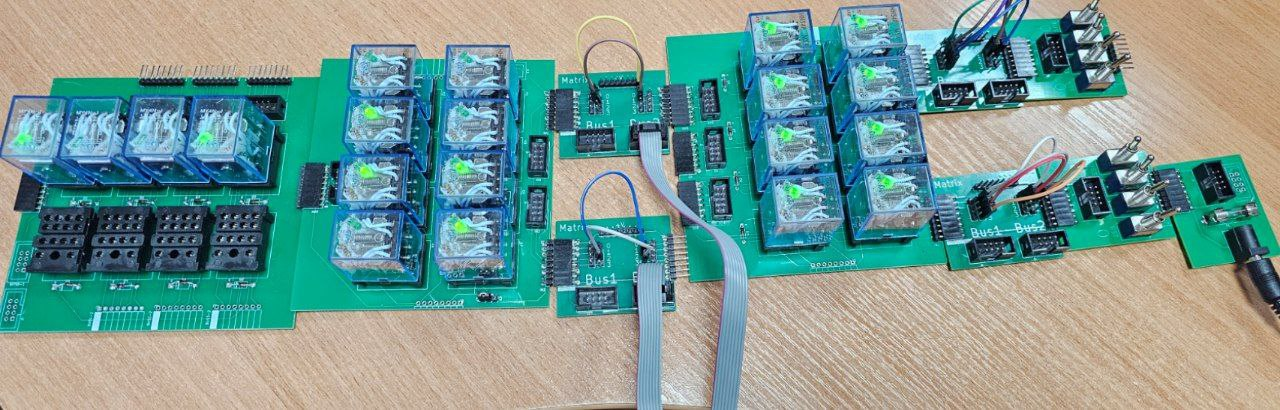
\includegraphics[width=\columnwidth]{photo/multiply.jpg}

Попробуйте набирать с помощью тумблеров разные значения для обоих
операндов (конечно же, они должны быть от~$0$ до~$3$) и проверьте,
правильный ли получается результат.

% R = A * B
% R0 = A0 & B0
% R1 = A1 & B0
% R2 = A0 & B1
% R3 = A1 & B1
% R = R0 + (R1 + R2) << 1 + R3 << 2

% R = A & B0 + (A << 1) & B1
% R = R1R0 + R3R2<0>

% Логический модуль для AND
% Сумматор для получения результата
% Несколько модулей для замешивания битов

\section{Калькулятор для пошагового деления}

Деление одного целого числа на другое будет простым только в случае,
если второе число это степень двойки. Например, при делении на $100_2$
мы просто отбрасываем две младшие двоичные цифры делимого.

Если же делитель не равен степени двойки, схема сильно усложняется.
Поэтому в первых микропроцессорах инструкции деления не существовало
и программистам приходилось писать для таких вычислений отдельную подпрограмму.

\section{Задачи}

\begin{enumerate}
    \item Соберите схему для вычитания двух чисел из соответствующей главы.
    \item Выполните деление числа $14$ на $3$ с помощью последовательности вычитаний.
          Записывайте промежуточные результаты на бумаге.
    \item Сделайте то же самое, только добавьте к схеме два регистра, чтобы результат очередного
          вычитания снова подать на вход сумматора.
\end{enumerate}

